\chapter{What Communication Requires}

This chapter follows J. Krishnamurti's 1974 San Diego dialogue with Allan W. Anderson on communication, relationship, seriousness, responsibility, and negation. The source is spoken inquiry, not a blackboard derivation; no validated board images or equations survive for this lecture. We will therefore use equations only as compact maps of the movement of the dialogue, keeping them visibly subordinate to the inquiry itself. Credit belongs to J. Krishnamurti and the Krishnamurti Foundation Trust source material, with curation by LazyingArt LLC through Video2Book.

\section{The Right Beginning}

Anderson begins by recalling a discipline from the previous conversation: do not complete a theory before one has found the right beginning. This matters because the present question is not merely, What is communication? It is communication and relationship together. The beginning is already relational.

Krishnamurti's first distinction is simple but decisive. Communication is not one person making a statement while the other accepts, rejects, compares, or stores it. Communication requires that we be engaged in the same movement of inquiry.

A compact way of recording the first movement is
\begin{equation}
\text{communication}
\approx
\text{verbal understanding}
+
\text{non-verbal communion}.
\end{equation}
This is not a formal equation from a board. It is a notation for the shape of the dialogue: words matter, but words alone are not communication.

The verbal side is ordinary enough. Two people speak a common language and understand the meanings of the words more or less. The non-verbal side is the harder condition: attention, listening, and a sharing of the problem while it is being unfolded.

\begin{definition}
In this chapter, \emph{communication} means the simultaneous movement of speaking, listening, sharing, and observing together. It is not mere information transfer, and it is not delayed agreement or disagreement.
\end{definition}

This definition must be read dynamically. Communication is not a state one enters after the discussion has succeeded. It is the condition of inquiry from the beginning.

\section{Listening As Shared Attention}

The word communication quickly opens into the art of listening. Krishnamurti's emphasis is not on interpretation but on attention. Real listening has no immediate movement of acceptance, denial, comparison, or judgment. It is the act of being with what is said and what is being investigated.

The dialogue gives us a useful simultaneity condition:
\begin{equation}
\text{same level}
+
\text{same time}
+
\text{same intensity}
\Longrightarrow
\text{walking together}.
\end{equation}
The phrase ``walking together'' is not decorative. It prevents a false model of communication in which one speaks, the other stores the statement, and only later begins to think. Krishnamurti is describing concurrent activity.

We can write the inner chain as
\begin{equation}
\text{listening}
\xrightarrow{\ \text{attention}\ }
\text{insight}.
\end{equation}
The important point is that insight is not placed at the end as a reward. It appears, if it appears at all, as the inquiry proceeds. Anderson recognizes this when he says that the insight is at the beginning, not at the end.

\begin{figure}
\centering
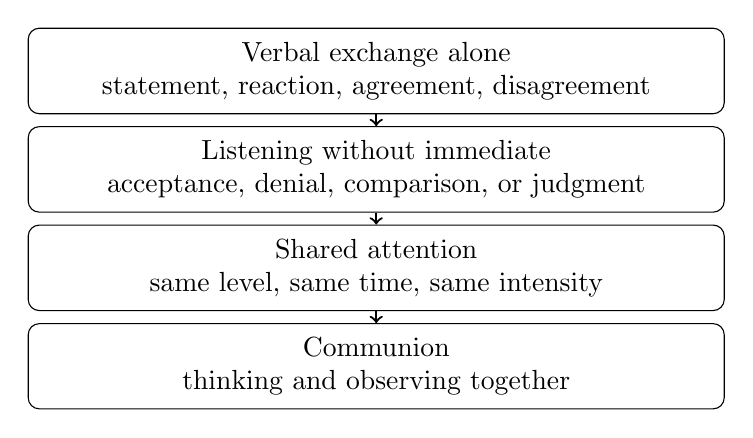
\begin{tikzpicture}[
  node distance=0.9cm,
  every node/.style={draw, rounded corners, align=center, text width=0.70\linewidth, inner sep=5pt},
  arrow/.style={->, thick}
]
\node (a) {Verbal exchange alone\\statement, reaction, agreement, disagreement};
\node (b) [below of=a, yshift=-0.35cm] {Listening without immediate\\acceptance, denial, comparison, or judgment};
\node (c) [below of=b, yshift=-0.35cm] {Shared attention\\same level, same time, same intensity};
\node (d) [below of=c, yshift=-0.35cm] {Communion\\thinking and observing together};
\draw[arrow] (a) -- (b);
\draw[arrow] (b) -- (c);
\draw[arrow] (c) -- (d);
\end{tikzpicture}
\end{figure}

This diagram is an editorial reconstruction from the transcript. It should not be mistaken for a system. It is only a pocket-sized way of preserving the sequence: from words, to listening, to attention, to communion.

\section{Seriousness Without Grimness}

The next turn is motivated by a difficulty in the word ``serious.'' Anderson notes that ordinary usage often makes seriousness sound like pain, heaviness, or the grim pursuit of a result. Krishnamurti refuses that meaning. A serious person is not necessarily long-faced or miserable. Seriousness means that the problem is real and must be met.

The analogy is direct. If one has cancer, one does not play with it. The seriousness is not psychological decoration; it belongs to the fact that the thing has to be understood and acted upon.

\subsection{Question \& Answer}

\paragraph{Question.}
Does seriousness mean effort stretched out over time?

\paragraph{Answer.}
No. In the dialogue, seriousness is not the promise that one will act later. It is the quality of seeing the problem as actual. When the seriousness is real, action is not postponed.

The contrast can be written as
\begin{equation}
\text{doing} \neq \text{``I will do''}.
\end{equation}
The phrase ``I will do'' already introduces psychological time. It moves away from the fact and into postponement. Krishnamurti's claim is sharper:
\begin{equation}
\text{clear seeing}
\Longrightarrow
\text{immediate action}.
\end{equation}

\begin{proposition}
For Krishnamurti, seriousness is not a mood but the inseparability of seeing and action before a real crisis.
\end{proposition}

\begin{proof}
The dialogue first rejects seriousness as pain, grimness, or wanting something from the problem. It then places seriousness in relation to the world as a disorder for which the human being is responsible. A serious problem is not deferred. Therefore the action appropriate to seriousness is immediate, not the delayed action of an ideal future.
\end{proof}

\section{Responsibility As Adequate Response}

Anderson then selects one element inside seriousness: responsibility. He hears the word as the capacity to be responsive. Krishnamurti accepts the direction and sharpens it: responsibility means responding adequately to a challenge.

The challenge is not abstract. The world is confused, sorrowful, violent, and disorderly. The human being has helped create this disorder. To be responsible is not to feel guilty in a vague way, and not to devise a plan from outside the problem. It is to respond to the problem itself.

A compact definition is
\begin{equation}
\text{responsibility}
=
\text{adequate response to challenge}.
\end{equation}
The danger is that we rarely respond to the challenge. We respond to our conclusion about the challenge. A plan is superimposed; if it fails, we blame ourselves or change the plan. But the plan has already displaced the fact.

The structure of this displacement is
\begin{equation}
\text{challenge}
\xrightarrow{\ \text{conclusion, plan, fear, pleasure, past}\ }
\text{translated response}
\neq
\text{adequate response}.
\end{equation}

\begin{figure}
\centering
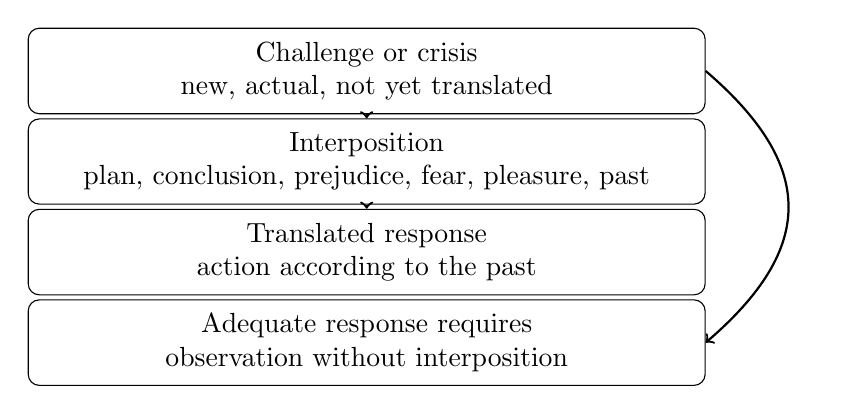
\begin{tikzpicture}[
  node distance=0.85cm,
  every node/.style={draw, rounded corners, align=center, inner sep=5pt},
  wide/.style={text width=0.68\linewidth},
  narrow/.style={text width=0.48\linewidth},
  arrow/.style={->, thick}
]
\node[wide] (challenge) {Challenge or crisis\\new, actual, not yet translated};
\node[wide, below of=challenge, yshift=-0.30cm] (screen) {Interposition\\plan, conclusion, prejudice, fear, pleasure, past};
\node[wide, below of=screen, yshift=-0.30cm] (response) {Translated response\\action according to the past};
\node[wide, below of=response, yshift=-0.30cm] (adequate) {Adequate response requires\\observation without interposition};
\draw[arrow] (challenge) -- (screen);
\draw[arrow] (screen) -- (response);
\draw[arrow] (challenge.east) .. controls +(1.4,-1.2) and +(1.4,1.2) .. (adequate.east);
\end{tikzpicture}
\end{figure}

This is the lecture's first major structural problem. If the response passes through the old machinery of conclusion, inclination, fear, pleasure, or belief, then the response is not adequate. It is a translation.

\section{The Observer Is The Observed}

The inquiry now reaches the claim that would be easy to treat as a slogan if we lifted it out of sequence. It is not introduced abstractly. It appears because the attempt to solve the problem from outside the problem has failed.

Krishnamurti says: the observer is the observed. In compact notation,
\begin{equation}
\text{observer} = \text{observed}.
\end{equation}
This is not mathematics in the ordinary sense. It is a way of refusing the separative posture in which one says, ``I am here, and the problem is over there.'' The human being has created the society he now observes. The disorder is not wholly external to him.

The related formulation is
\begin{equation}
\text{world} = \text{me},
\qquad
\text{me} = \text{world}.
\end{equation}
Krishnamurti insists that this is not to be taken as an intellectual or emotional statement. Within the dialogue it functions as a fact to be seen: human beings, irrespective of labels such as nationality, share the same problems of relationship, suffering, jealousy, greed, ambition, imitation, and conformity.

This changes the character of response. If the observer is separate from the observed, action is partial. The observer tries to operate upon a problem outside himself. But if the observer is the observed, then change, if it happens, is total. The one who would fix the problem is implicated in the problem.

\begin{remark}
The chapter should not turn this into metaphysics. The claim belongs to the local argument about responsibility: we cannot respond adequately while maintaining the fiction that the disorder is merely outside us.
\end{remark}

\section{Learning From The Problem}

Anderson then raises the practical objection that gives this part of the dialogue its force. A person may say: I hear this, I have some intuition of it, but what am I to do? If I open myself to the crisis, everything seems to rush in. If I must begin, where do I begin?

\subsection{Question \& Answer}

\paragraph{Question.}
What is a human being to do when confronted with suffering, chaos, and violence?

\paragraph{Answer.}
Krishnamurti's answer is not a method. One must learn from the problem itself. That requires humility: the mind must not come saying, ``I know.'' It must come to the problem without conclusion, without prearranged solution, without a plan borrowed from the past.

The essential identity is
\begin{equation}
\text{learning} = \text{doing}.
\end{equation}
This identity is one of the chapter's central pieces. It rules out the comforting idea that one possesses a capacity that will someday actualize itself. The learning is not preparation for action. The learning is the action.

We can set the reasoning as a short derivation.

\begin{enumerate}
\item The human being confronts a fact: disorder, suffering, violence, confusion.
\item If he approaches the fact with a conclusion, he has already translated it.
\item Translation by the past prevents direct learning from the fact.
\item Therefore the first requirement is humility: ``I do not know.''
\item With no conclusion imposed, the fact itself can be observed and listened to.
\item In that observation, learning and doing are not two movements.
\end{enumerate}

This is why Krishnamurti says that the problem itself will reveal a great deal if one is capable of looking at it. The answer is not brought to the problem; the fact must be allowed to disclose itself.

\section{Negation, Attention, And The Positive}

The conversation then turns through a sentence Anderson reads from \emph{The Awakening of Intelligence}: through negation, that which alone is positive comes into being. Anderson hears that something is done through negation; Krishnamurti agrees. This is important, because the lecture is not saying that words are useless and therefore one should retreat into vagueness. There is an act.

The compact relation is
\begin{equation}
\text{actual negation}
\Longrightarrow
\text{the positive comes into being}.
\end{equation}
But the word ``negation'' is dangerous. Anderson senses a double aspect: desire for success already withholds one from the problem, and that withholding is itself a kind of negation. Krishnamurti clarifies the matter. Negation, as commonly understood, may mean violence: brushing aside, suppressing, rejecting. That is not the meaning here.

\begin{definition}
\emph{Actual negation} means understanding the whole movement of what is false, immoral, or separative, so that it ends. It is not verbal denial, violent rejection, sacrifice, or punishment.
\end{definition}

The first example is society's immorality:
\begin{equation}
\text{negation of immorality}
\Longrightarrow
\text{morality}.
\end{equation}
The second example is success. Krishnamurti includes worldly success and so-called spiritual success together: money, position, authority, achievement, and spiritual ambition belong to the same field when they are movements of becoming and power.

The structure of the example is
\begin{align}
\text{attention to success}
&\Longrightarrow
\text{the whole map of success is revealed},\\
\text{the whole map is seen}
&\Longrightarrow
\text{success as motive ends},\\
\text{success as motive ends}
&\Longrightarrow
\text{different action}.
\end{align}
The ``map'' includes ruthlessness, lack of love, lack of consideration, conformity, imitation, acceptance of the social structure, and the desire for power or prestige. Negating success is not an act of violence. It is an act of tremendous attention.

\begin{figure}
\centering
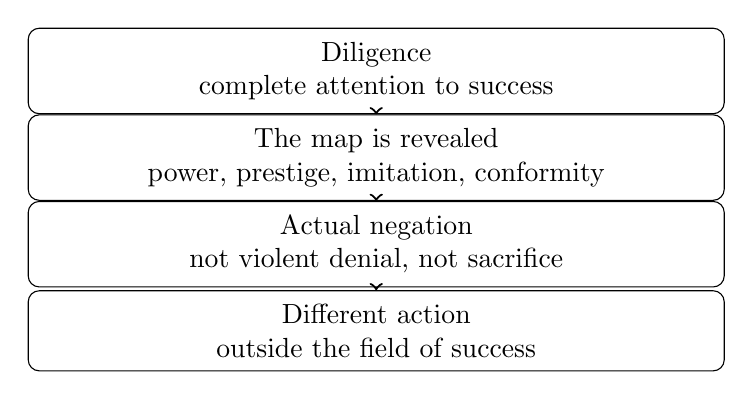
\begin{tikzpicture}[
  node distance=0.8cm,
  every node/.style={draw, rounded corners, align=center, text width=0.70\linewidth, inner sep=5pt},
  arrow/.style={->, thick}
]
\node (a) {Diligence\\complete attention to success};
\node (b) [below of=a, yshift=-0.30cm] {The map is revealed\\power, prestige, imitation, conformity};
\node (c) [below of=b, yshift=-0.30cm] {Actual negation\\not violent denial, not sacrifice};
\node (d) [below of=c, yshift=-0.30cm] {Different action\\outside the field of success};
\draw[arrow] (a) -- (b);
\draw[arrow] (b) -- (c);
\draw[arrow] (c) -- (d);
\end{tikzpicture}
\end{figure}

This also clarifies why Krishnamurti is wary of the inherited term ``self-denial.'' If self-denial means sacrifice, pain, or religious punishment, it distorts clear perception. If something is seen clearly, the action is immediate. One does not need to keep up an act of denial. Seeing danger is enough not to go near it.

\section{Responsibility Without Delegation}

The final movement returns to responsibility in relationship. The conversation turns to the widespread habit of delegation: politicians, priests, analysts, psychologists, professors, religious authorities, and traditions are made responsible, while the person says, in effect, ``I only follow.'' Krishnamurti calls this irresponsibility.

The rule can be written plainly:
\begin{equation}
\text{delegated responsibility}
\Longrightarrow
\text{irresponsibility}.
\end{equation}
Responsibility means total commitment to the challenge. A challenge is new; otherwise it is not a challenge. A crisis is new; otherwise it is not a crisis. Therefore the past cannot respond adequately to it.

The closing obstruction list is severe:
\begin{equation}
\text{fear}
\lor
\text{pleasure}
\lor
\text{routine}
\lor
\text{tradition}
\lor
\text{conditioning}
\Longrightarrow
\text{incomplete response}.
\end{equation}
And the final condition is
\begin{equation}
\text{adequate response to challenge}
\Longrightarrow
\text{ending of the me as past}.
\end{equation}

Anderson's example from the \emph{Bhagavad Gita} is used to sharpen the point. Arjuna asks to be told definitely what to do. In this reading, the request itself can be a refusal of responsibility. To ask another to carry the act of seeing for me is already to remain in the past. Responsibility is not obedience to an answer; it is total response to the challenge.

\section{Summary}

The chapter has moved in the same order as the dialogue. Communication begins as a question about words, but it quickly becomes a question about listening. Listening requires attention; attention opens the possibility of insight; insight is not delayed until the end. Communication becomes communion when two people meet the same problem with the same seriousness.

Seriousness is then separated from grim effort. It means total responsibility before an actual crisis. Responsibility is not the application of a plan, conclusion, belief, fear, pleasure, or tradition. It is adequate response to a challenge. That is why the observer cannot remain outside the observed: the world one tries to correct is not separate from the human being who has helped create it.

Finally, negation is shown to be neither suppression nor sacrifice. Actual negation is the seeing of the whole movement of success, power, immorality, or separation. In that seeing, the false thing ends; action is no longer in the old field. The lecture closes by refusing delegation. To respond completely, the self as past must end.